\textbf{Задание №4} Написать программу, которая определяет, можно ли применить заданную последовательность правил р при выводе терминальной цепочки в заданной КС-грамматике и формирует линейную скобочную
    форму дерева вывода. Если последовательность правил р можно применить при выводе v терминальной цепочки, то программа должна вывести последовательность правил, применяемую при левом выводе, эквивалентном выводу v. Обработать программой последовательность правил, найденную в п.3.
    Примечание. Если к нетерминалу А в процессе вывода применяется
    правило с номером n, то в линейной скобочной форме дерева вывода после нетерминала А должен быть символ с кодом n. \label{sec:4}

    \begin{minted}[style=xcode, frame=lines, framesep=2mm, baselinestretch=1.2, fontsize=\small, linenos]{cpp}
#include <iostream>
#include <string>
#include <vector>
#include <cctype>
using namespace std;

const char lhs[9]   = {' ', 'S', 'S', 'S', 'A', 'A', 'A', 'B', 'B'};
const string rhs[9] = {"", "Aba", "bS", "cAbA", "AaS", "BaB", "e", "b", "aA"};

bool isNonterminal(char c)
{
    return isupper(static_cast<unsigned char>(c)) != 0;
}

bool isDigitChar(char c)
{
    return isdigit(static_cast<unsigned char>(c)) != 0;
}

string applyRule(const string& form, int pos, int rule)
{
    return form.substr(0, pos) + rhs[rule] + form.substr(pos + 1);
}

int countNonterminalsBefore(const string& form, int pos)
{
    int cnt = 0;
    for (int i = 0; i < pos && i < (int)form.size(); ++i)
        if (isNonterminal(form[i]))
            ++cnt;
    return cnt;
}

int findKthStar(const string& lsf, int k)
{
    int cnt = 0;
    for (int i = 0; i < (int)lsf.size(); ++i)
    {
        if (lsf[i] == '*')
        {
            if (cnt == k)
                return i;
            ++cnt;
        }
    }
    return -1;
}

string expandRuleForLsf(char nonTerm, int rule)
{
    string repl = string(1, nonTerm) + "(" + to_string(rule) + ")(";
    const string& r = rhs[rule];

    for (int i = 0; i < (int)r.size(); ++i)
    {
        if (i > 0)
            repl += " ";

        char c = r[i];

        if (c == 'e')
            repl += "ε";
        else if (isNonterminal(c))
        {
            repl += '*';
            repl += c;
        }
        else
            repl += c;
    }

    repl += ")";
    return repl;
}

string updateLsf(const string& lsf, int k, char nonTerm, int rule)
{
    int starPos = findKthStar(lsf, k);
    if (starPos < 0)
        return lsf;

    return lsf.substr(0, starPos) + expandRuleForLsf(nonTerm, rule) 
           + lsf.substr(starPos + 2);
}

string cleanLsf(const string& lsf)
{
    string s;
    for (char c : lsf)
        if (c != '*')
            s += c;
    return s;
}

bool hasNonterminals(const string& form)
{
    for (char c : form)
        if (isNonterminal(c))
            return true;
    return false;
}

void printRuleSequence(const vector<int>& p)
{
    cout << "Последовательность правил p: ";
    for (int r : p)
        cout << r << " ";
}

bool search(const vector<int>& p, int step, const string& form, vector<int>& positions)
{
    if (step == (int)p.size())
        return !hasNonterminals(form);

    char need = lhs[p[step]];

    for (int i = 0; i < (int)form.size(); ++i)
    {
        if (form[i] != need)
            continue;

        string next = applyRule(form, i, p[step]);
        positions.push_back(i);

        if (search(p, step + 1, next, positions))
            return true;

        positions.pop_back();
    }

    return false;
}

string buildLsf(const vector<int>& p, const vector<int>& positions)
{
    string form = "S";
    string lsf  = "*S";

    for (int step = 0; step < (int)p.size(); ++step)
    {
        int rule = p[step];
        int pos  = positions[step];
        int k    = countNonterminalsBefore(form, pos);
        char nonTerm = form[pos];

        lsf  = updateLsf(lsf, k, nonTerm, rule);
        form = applyRule(form, pos, rule);
    }

    return lsf;
}

string getTerminalChain(const vector<int>& p, const vector<int>& positions)
{
    string form = "S";

    for (int step = 0; step < (int)p.size(); ++step)
        form = applyRule(form, positions[step], p[step]);

    string result;
    for (char c : form)
        if (c != 'e')
            result += c;

    return result;
}

bool matchRuleAt(const string& lsf, int i, int& rule, int& nextPos)
{
    if (!isNonterminal(lsf[i]))
        return false;

    if (i + 1 >= (int)lsf.size() || lsf[i + 1] != '(')
        return false;

    int j = i + 2;
    int r = 0;

    while (j < (int)lsf.size() && isDigitChar(lsf[j]))
    {
        r = r * 10 + (lsf[j] - '0');
        ++j;
    }

    if (j >= (int)lsf.size() || lsf[j] != ')')
        return false;

    rule = r;
    nextPos = j + 1;
    return true;
}

vector<int> extractLeftmost(const string& lsf)
{
    vector<int> seq;

    for (int i = 0; i < (int)lsf.size(); ++i)
    {
        int rule = 0;
        int nextPos = i;

        if (matchRuleAt(lsf, i, rule, nextPos))
        {
            seq.push_back(rule);
            i = nextPos - 1;
        }
    }

    return seq;
}

int main()
{
    vector<int> p = {2, 2, 2, 1, 4, 2, 5, 7, 7, 1, 6};

    printRuleSequence(p);
    cout << "\n";

    vector<int> positions;

    if (search(p, 0, "S", positions))
    {
        cout << "Последовательность применима при произвольном выводе.\n";

        string lsf = buildLsf(p, positions);
        cout << "ЛСФ дерева вывода:\n" << cleanLsf(lsf) << "\n";

        vector<int> leftSeq = extractLeftmost(lsf);
        cout << "Последовательность правил при левом выводе, "
                "эквивалентном v: ";
        for (int r : leftSeq)
            cout << r << " ";
        cout << "\n";

        cout << "Терминальная цепочка: "
             << getTerminalChain(p, positions) << "\n";
    }
    else
    {
        cout << "Последовательность не применима "
                "при произвольном выводе.\n";
    }

    return 0;
}
    \end{minted}
    

    \begin{figure}[H]
        \centering
        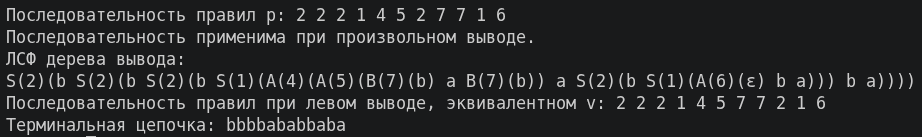
\includegraphics[width = 1 \textwidth]{picture/exercise4.png}
        \caption{Результат выполнения программ}
    \end{figure}